% !TeX root = ../Report.tex
\chapter{Proof of Concept Evaluation}
\label{sec:poc evaluation}

\section{Evaluation Objectives}
\label{sec:evaluation objectives}

The objective of the Proof of Concept (PoC) evaluation is to assess the ability of FUNES to provide context-aware decision support in a representative Earth Observation ground segment scenario. The evaluation focuses on the core capabilities introduced by the proposed architecture, with particular emphasis on the retrieval and integration of heterogeneous operational information, the identification of anomalies and their operational impact, and the generation of appropriate decision-support outputs.

The evaluation is structured to progressively assess the capabilities required by FUNES to support mission operators. At a first level, the evaluation considers the ability of the system to retrieve relevant information from individual operational sources. At a second level, it assesses the ability to correlate information originating from different mission domains, such as network monitoring, incident management, and mission planning. Finally, more complex tasks are considered, requiring the system to combine information from multiple sources, identify the resulting operational risks, and provide recommendations consistent with the available evidence and with the role of a Decision Support System.

A further objective is to assess the contribution of the proposed retrieval and multi-agent orchestration approach with respect to a general-purpose Large Language Model operating directly on the complete operational context. For this purpose, the responses generated by FUNES are compared with those produced by a baseline LLM (llama 3.3 70b instruct) under the same operational scenario. The comparison is intended to evaluate whether the system architecture can improve the ability to identify relevant information, correlate operational evidence, and provide decision-support outputs while limiting the amount of contextual information that must be supplied to the underlying language model.

The evaluation therefore addresses the following main objectives:

\begin{itemize}
\item assess the capability of FUNES to retrieve relevant information from heterogeneous operational sources;
\item evaluate the ability to correlate information across different mission domains;
\item assess the identification of operational anomalies and their impact on planned satellite activities;
\item evaluate the accuracy of planning-related information and the identification of affected operations;
\item assess the ability of the system to filter irrelevant information and focus on the elements relevant to the operator's query;
\item evaluate whether the generated outputs are consistent with the role of a Decision Support System, supporting rather than replacing human decision-making;
\item assess the quality and operational consistency of the recommendations generated for complex scenarios;
\item compare the resulting decision-support performance with that of a general-purpose LLM provided with the complete operational context.
\end{itemize}

The evaluation is intended as a validation of the PoC capabilities rather than as a comprehensive validation of a production-ready operational system. Consequently, the results are interpreted in terms of the feasibility and effectiveness of the proposed approach within the considered representative scenario, rather than as a general measure of system performance across all possible mission operational conditions.


\section{Evaluation Scenario}
\label{sec:evaluation scenario}

A representative Earth Observation ground segment scenario was defined to evaluate the Proof of Concept under operational conditions requiring the analysis and correlation of heterogeneous information sources. The scenario, depicted in Fig. \ref{fig:evaluation_scenario}, was designed to reproduce, at a simplified level, the type of information fragmentation that characterizes a real mission operations environment, where the assessment of an operational situation may require information from mission planning, network monitoring, incident management, and mission knowledge sources.

The scenario includes three ground stations, namely GS-01, GS-02, and GS-03, and four satellites, namely SAT-01, SAT-02, SAT-03, and SAT-04. SAT-01 is nominally served by GS-01, SAT-02 and SAT-03 by GS-02, and SAT-04 by GS-03. GS-01 is additionally connected to GS-02 and GS-03 through inter-station network links, introducing dependencies between the operational status of different ground stations.

The operational context was constructed from four main information domains: mission planning, network monitoring, incident and change management, and mission knowledge. The resulting scenario provides both nominal operational information and intentionally introduced anomalies, allowing the evaluation to consider not only direct information retrieval but also cross-domain correlation and operational impact analysis.


\begin{figure}
    \centering
    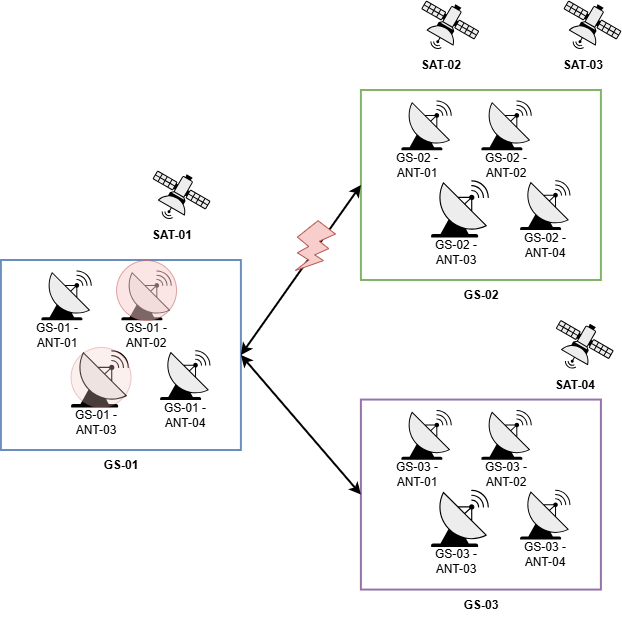
\includegraphics[width=0.6\textwidth]{Figures/funes_scenario.png}
    \caption{Overview of the evaluation scenario: the are 3 ground segment stations GS-01, GS-02, and GS-03, each with 4 antennas, and 4 satellites SAT-01, SAT-02, SAT-03, and SAT-04. The GS-01 is connected to both GS-02 and GS-03 through inter-station network links. The link between GS-01 and GS-02 is degraded, while the link between GS-01 and GS-03 is operational but exhibits increased latency. The GS-01/ANT-02 is unavailable, while GS-01/ANT-03 is degraded. The remaining antennas of GS-01 are operational, while GS-02 and GS-03 are nominal at station level. The ANT positioning is close to the respective ground stations.}
    \label{fig:evaluation_scenario}
\end{figure}


\subsection{Mission Planning}

For each satellite, approximately 36 hours of mission planning data were generated around the evaluation period. The planning information is structured as a sequence of satellite passages, with each passage associated with a ground station and a set of scheduled activities. Each activity contains its type, temporal interval, and the antenna on which it is scheduled.

The activities are not identical across passages and may include different operational types, such as uplink (UPL) and downlink (DWL) operations. This variability was introduced to provide a realistic planning context in which the impact of an unavailable resource cannot be determined solely from the satellite or ground station identifier, but requires inspection of the actual scheduled activities and their temporal characteristics.

The planning dataset therefore enables questions involving different levels of temporal and operational reasoning, including the retrieval of the next satellite pass, identification of scheduled activities, identification of affected acquisitions, and assessment of potential planning conflicts.

\subsection{Ground Segment and Network Status}

The scenario contains network monitoring information for all three ground stations and their associated antennas. For each station, the network data include the overall station status, backhaul capacity and utilization, average latency, and packet loss. At antenna level, the status, throughput, latency, packet loss, and utilization are provided.

The network scenario intentionally includes different operational conditions. GS-01 is in a degraded overall state, with antenna ANT-02 offline and ANT-03 exhibits increased latency and packet loss. The remaining antennas of GS-01 are operational. GS-02 and GS-03 are nominal at station level, although their individual resource utilization differs.

Inter-station connectivity is also included in the scenario. The connection between GS-01 and GS-02 is degraded, with reduced available bandwidth, increased latency, and packet loss. The connection between GS-01 and GS-03 is reported as operational in terms of connectivity status, but exhibits a significantly higher latency. These conditions introduce additional information that must be interpreted and filtered in relation to the actual operational activities and user questions rather than treated independently.

This configuration was deliberately designed to avoid a scenario in which the presence of an anomaly directly determines its operational consequence. For example, detecting that an antenna is unavailable is not sufficient to determine whether satellite operations are affected. The corresponding planning information must also be examined to identify the activities scheduled on the affected resource.

\subsection{Operational Events and Tickets}

The scenario includes a set of operational events representing anomalies, maintenance activities, and external operational requests. These events generate different types of operational records, including incident tickets, change tickets, and customer requests.

The main events include the unavailability of GS-01/ANT-02, degradation of the connectivity between GS-01 and GS-02, planned preventive maintenance on GS-02/ANT-02, and an additional customer acquisition request for the busy satellite SAT-01 of GS-01. These events have been associated with potential impacts on scheduled satellite activities, allowing the system to assess the relationship between an operational event and its consequences on mission planning.

To reproduce the presence of unrelated information typically encountered in operational environments, the scenario contains 32 tickets in total. Only six of these tickets are directly relevant to the operational events introduced in the scenario, while the remaining tickets describe plausible but unrelated operational issues and ground segments events. These additional records act as contextual noise and require the system to distinguish information relevant to the current operational situation from unrelated historical or concurrent events.

The inclusion of irrelevant but plausible tickets is particularly important for the evaluation of a decision-support system. In a realistic operational environment, the presence of a large amount of available information does not imply that all information is relevant to a given operator query. The ability to identify and filter the relevant evidence is therefore considered an integral part of the evaluation scenario.

\subsection{Mission Knowledge Base}

The scenario is complemented by a knowledge base containing 20 documents covering mission and system information. These documents provide contextual knowledge that is not directly represented in the operational planning, network, or ticket data.

The knowledge base is used to support questions requiring background information about the mission and its systems, as well as questions in which operational observations need to be interpreted using previously defined system knowledge. Its inclusion allows the evaluation to distinguish between direct retrieval of operational data and the use of persistent domain knowledge during the reasoning process.

\subsection{Scenario Design Rationale}

The scenario was deliberately constructed to reproduce the main characteristics that motivate the FUNES architecture: heterogeneous information sources, temporal dependencies, operational anomalies, cross-domain relationships, and the presence of irrelevant information.

A scenario based exclusively on isolated retrieval questions would not adequately test the capabilities targeted by the PoC. For example, identifying that an antenna is offline is a relatively simple retrieval task. Determining whether this condition affects a satellite operation, however, requires the system to correlate the network status with the mission planning and to identify the activities assigned to the affected resource. Similarly, determining whether an operational issue requires immediate attention may require the combination of anomaly information, incident records, mission planning, and domain knowledge.

For this reason, the scenario was designed with increasing levels of information dependency. Some questions can be answered using a single information source, while others require the correlation of two or more sources. The most complex questions require the integration of multiple operational domains to identify current risks and formulate appropriate decision-support recommendations.

The presence of both relevant and irrelevant information was also intentional. The objective was not to create an artificially clean dataset in which every available record contributes to the answer, but to approximate the information overload encountered in operational environments. This allows the evaluation to consider not only whether FUNES can retrieve information, but also whether it can identify the information that is relevant to the specific operational question.

Overall, the scenario was designed to provide a controlled but sufficiently heterogeneous environment in which the principal capabilities of the proposed FUNES architecture can be exercised: retrieval of mission knowledge and operational data, correlation of information across different sources, identification of operational impacts, and generation of decision-support outputs.


\section{Evaluation Tasks and Experimental Setup}
\label{sec:evaluation tasks and setup}

The evaluation was designed around a set of operational questions derived from a representative ground segment scenario. The questions were defined to progressively increase in complexity and to exercise the main capabilities provided by the FUNES architecture. In particular, three levels of task complexity were considered: single-source retrieval, multi-source correlation, and decision-support tasks.

\subsection{Evaluation Tasks}

The first category consists of \textit{easy tasks}, which require the retrieval of information from a single operational source. These tasks are intended to verify the basic ability of the system to identify the appropriate information source and retrieve the relevant information. The considered sources include the knowledge base, mission planning, network monitoring, and incident management systems. Representative questions include queries regarding the architecture and operational interfaces of the Flight Operations System, the current network status, the status of a ground-station antenna, currently open incidents, and the next scheduled satellite passes.

The second category consists of \textit{medium tasks}, which require the retrieval and correlation of information from multiple operational sources. These tasks are designed to evaluate whether the system can combine heterogeneous information to derive operationally relevant conclusions. For example, determining why a ground station is unavailable requires the correlation of network information with incident records, while identifying the satellite acquisitions affected by an incident requires information from both the incident management and mission planning domains. Other tasks require the system to determine whether a ground station is available for a planned acquisition or whether an acquisition can be rescheduled based on the available planning information.

The third category consists of \textit{hard tasks}, which extend the previous category by requiring situational assessment and decision support. These tasks require the system to integrate information from multiple operational sources, identify relevant anomalies, determine their impact on mission activities, and, where appropriate, propose possible operational actions. Examples include identifying the current operational issues affecting the ground segment, determining which issues require immediate attention, identifying risks to planned activities for a given operational day, and summarizing current anomalies together with their operational impact and possible mitigation actions.

This progressive organization allows the evaluation to distinguish between the ability to retrieve individual pieces of information and the higher-level capabilities required for operational decision support. The complete set of evaluation questions is reported in Table~\ref{tab:evaluation questions}.

\subsection{Experimental Setup}

The evaluation was conducted by comparing the responses generated by the FUNES PoC with those produced by a general-purpose Large Language Model used as a baseline. FUNES was evaluated using its complete processing pipeline, including the selection of the appropriate information sources, retrieval of the relevant operational context, correlation of the retrieved information, and generation of the final response.

As a baseline, \textit{Llama 3.3 70B Instruct} was provided with the complete operational context associated with the evaluation scenario. In contrast to FUNES, the baseline did not perform explicit source selection or selective retrieval. Instead, the entire available context was provided directly to the model together with the user query. This configuration was selected to provide a reference for assessing the contribution of the retrieval and orchestration mechanisms implemented by FUNES.

The two systems were evaluated using the same set of operational questions and the same underlying scenario. For each question, the generated response and, for FUNES, the information sources selected during the reasoning process were recorded. This allowed the evaluation to consider both the quality of the final answers and the behaviour of the underlying information-selection mechanism.

In addition to the generated answers, the amount of contextual information provided to the language model was recorded in terms of input tokens. This measurement was used to investigate whether the selective retrieval strategy adopted by FUNES can reduce the amount of operational context supplied to the underlying language model while maintaining effective decision-support capabilities.

The resulting evaluation therefore considers two complementary aspects of the proposed architecture. First, the quality of the decision-support responses is assessed across tasks with increasing levels of complexity. Second, the behaviour of the information retrieval and orchestration mechanisms is analysed by considering tool selection and contextual input requirements. This setup provides a basis for evaluating not only whether the system produces appropriate answers, but also whether the architectural mechanisms introduced by FUNES contribute to the observed behaviour.


\section{Evaluation Methodology}
\label{sec:evaluation methodology}

The evaluation was conducted through a scenario-based methodology designed to reproduce a representative operational situation within an Earth Observation ground segment. A predefined operational scenario was constructed by combining information from the knowledge base, ground station monitoring, network status, incident and change management, and mission planning. The scenario includes both nominal operational information and a set of concurrent operational events affecting the ground segment and scheduled satellite activities.

A set of predefined questions was then formulated to assess the decision-support capabilities of the PoC. The questions were organised according to three increasing levels of complexity. The first level consists of single-source retrieval tasks, requiring information to be obtained from a single operational subsystem. The second level consists of retrieval and correlation tasks, where information from multiple sources must be combined to answer the query. The third level consists of decision-support tasks, requiring the identification of multiple operational issues, the analysis of their potential impact on mission activities, and, where appropriate, the formulation of possible operational actions.

The evaluation was performed using two systems. The first system was the FUNES PoC, including its retrieval, tool-selection, multi-agent orchestration, and reasoning capabilities. The second system was a baseline based on the Llama 3.3 70B Instruct model. The baseline was provided with the complete operational context and was asked to answer the same questions without the selective retrieval and multi-source orchestration mechanisms implemented by FUNES. This configuration was selected to provide a comparison between the proposed architecture and a general-purpose LLM operating directly on the available operational context.

For each question, both systems generated an answer independently. The resulting answers were subsequently evaluated using an LLM-as-a-Judge \cite{zheng2023judging} approach. Google Gemini Flash 3.6 was employed as an independent evaluator and was provided with the operational context, the question, and the two generated answers. The evaluator was instructed to assess the responses with respect to the operational evidence contained in the scenario, without considering stylistic aspects such as response length or linguistic quality.

The evaluation criteria were defined to reflect the main capabilities expected from an operational Decision Support System. Each criterion was evaluated using a three-level ordinal scale:

\begin{itemize}
\item \textbf{0 Incorrect:} the answer contains false or misleading information, fails to identify relevant anomalies, establishes incorrect correlations, reports incorrect planning information, or proposes operational actions that are inconsistent with the available evidence;
\item \textbf{1 Correct but incomplete:} the answer contains no critical incorrect information but identifies only part of the relevant information, omits significant anomalies or impacts, or provides only a partial analysis;
\item \textbf{2 Fully correct:} the answer correctly identifies the relevant information and, where applicable, establishes the appropriate relationships between operational evidence, impacts, and possible actions.
\end{itemize}

The following criteria were considered in the evaluation:

\begin{itemize}
\item \textbf{Anomaly Identification}: measures the ability to identify the operational anomalies relevant to the question, including degraded or unavailable components, network issues, and active operational incidents;

\item \textbf{Evidence Correlation}: measures the ability to correctly connect information originating from different operational sources and derive relationships between events, anomalies, and their consequences;

\item \textbf{Planning Accuracy}: measures the correctness of planning-related information, including affected acquisitions, scheduled activities, available opportunities, and potential planning conflicts;

\item \textbf{Noise Filtering}: measures the ability to distinguish information relevant to the query from unrelated elements of the operational context, avoiding unnecessary or unsupported conclusions;

\item \textbf{DSS Role Adherence}: measures whether the generated response is consistent with the role of a Decision Support System. Responses are expected to provide evidence-based information and recommendations while supporting, rather than replacing, the human operator's decision-making process;

\item \textbf{Operational Action Quality}: measures the consistency and usefulness of proposed operational actions with respect to the available evidence, particularly for questions requiring mitigation or decision-support recommendations.


\end{itemize}

Not all evaluation criteria are applicable to every question. The applicable criteria depend on the information and reasoning capabilities required by the specific task. For example, a single-source network status query primarily evaluates information retrieval and anomaly identification, whereas a question concerning the impact of an incident on scheduled acquisitions requires evidence correlation and planning accuracy. Similarly, recommendation-oriented questions require the additional assessment of Decision Support System adherence and operational action quality. This criterion-dependent evaluation avoids penalising a response for not providing information or reasoning that was not required by the question.

In addition to the quality of the generated answers, the evaluation considered two system-level indicators. The first is \textbf{tool selection accuracy}, evaluated for questions requiring the use of FUNES tools or operational data sources. This metric measures whether the system selected the appropriate information sources required to answer the query. The second is the \textbf{average number of input tokens} provided to the underlying language model. This metric is used to compare the amount of contextual information supplied by FUNES with that supplied to the baseline, providing an indication of the effectiveness of selective information retrieval.

The LLM-as-a-Judge evaluator was instructed to evaluate the two responses independently with respect to the operational context and predefined criteria. The identities of the systems were not considered part of the evaluation criteria, and the assessment focused exclusively on the content and operational validity of the generated responses. For each question, the individual criterion scores were recorded and subsequently aggregated to enable comparison between FUNES and the baseline across the different task complexity levels and evaluation dimensions.

The use of an LLM-as-a-Judge was selected to provide a consistent evaluation procedure for responses where correctness cannot always be expressed through exact matching. In particular, complex decision-support questions may admit multiple valid formulations or operationally reasonable recommendations. The evaluator therefore assesses the consistency of each response with the evidence and operational constraints defined by the scenario rather than requiring an exact reference answer. To reduce potential evaluator bias related to the identity or position of the compared systems, the association between the two responses and the system identities was randomized during the evaluation.

The methodology is intended to provide a comparative evaluation of the PoC rather than a statistically exhaustive validation of an operational system. The results should therefore be interpreted within the scope of the considered scenario, question set, and evaluation procedure. In particular, the use of an external LLM as an evaluator introduces an additional source of potential evaluation bias, while the proprietary nature of the evaluator prevents complete inspection of its internal decision process. These aspects are considered when discussing the results and limitations of the evaluation.

The set of questions is reported in Table \ref{tab:evaluation_questions}, together with their corresponding identifiers. The questions are designed to progressively increase in complexity, with the first 10 questions classified as easy tasks (E), the next 6 (Q11-Q16) as medium tasks (M), and the final 4 (Q17-Q20) as hard tasks (H). 



\begin{table}[htbp]
\centering
\caption{Evaluation question set.}
\label{tab:evaluation_questions}
\begin{tabularx}{\textwidth}{cX} % <--- Imposta la larghezza pari alla pagina e la colonna X va a capo da sola
\hline
\textbf{ID} & \textbf{Question} \\
\hline
\textbf{Q1} & What are the architecture and operational interfaces of FOS for HR-MS satellites in the IRIDE ground segment? \\
\textbf{Q2} & How does FOS manage and interact with the HR-MS satellites in the IRIDE system? \\
\textbf{Q3} & What are the requirements and procedures for developing software validation specifications according to ECSS-E-ST-40? \\
\textbf{Q4} & When is satellite SAT-01 next pass on GS-01? \\
\textbf{Q5} & How many passes does satellite SAT-02 have on 2026-05-26 on GS-02? \\
\textbf{Q6} & What is the current network status? \\
\textbf{Q7} & Is the connection to antenna ANT-02 of GS-01 online? \\
\textbf{Q8} & Which incidents are currently open? \\
\textbf{Q9} & Is there an open ticket for GS-02? \\
\textbf{Q10} & Is there an open ticket regarding power supplies? \\
\midrule
\textbf{Q11} & Why is GS-01 degraded? \\
\textbf{Q12} & Which acquisitions are affected by incident INC-101? \\
\textbf{Q13} & Is the ground station assigned to SAT-02 available? \\
\textbf{Q14} & How many acquisitions are we going to lose if antenna ANT-01 is unavailable from 2026-05-26 10:00 to 2026-05-26 12:00? \\
\textbf{Q15} & When can SAT-01-PASS-032 be rescheduled according to its usual time schedule of past days? Give the next possible datetime. \\
\textbf{Q16} & Can the urgent acquisition request be accommodated? \\
\midrule
\textbf{Q17} & Provide an overview of the current operational issues and their impact on scheduled satellite operations. \\
\textbf{Q18} & What operational issues require immediate attention and what mitigation actions should be applied? \\
\textbf{Q19} & Identify risks for planned activities on 2026-05-26 and report the affected activities with their corresponding datetime. \\
\textbf{Q20} & Summarize the current anomalies, explain their operational impact and recommend the next possible operational actions. \\
\hline
\end{tabularx}
\end{table}






\begin{table}[htbp]
\centering
\caption{Information sources and task type associated with each evaluation question. \textbf{Legenda:} KB = Knowledge Base, MP = Mission Planning, NM = Network Monitoring, TM = Ticket Management.}
\label{tab:question_sources}
\renewcommand{\arraystretch}{1.1}
\begin{tabularx}{\textwidth}{c *{4}{>{\centering\arraybackslash}X} l}
\toprule
\textbf{ID} & \textbf{KB} & \textbf{MP} & \textbf{NM} & \textbf{TM} & \textbf{Task type} \\
\midrule
Q1  & X &   &   &   & Single-source retrieval \\
Q2  & X &   &   &   & Single-source retrieval \\
Q3  & X &   &   &   & Single-source retrieval \\
Q4  &   & X &   &   & Single-source retrieval \\
Q5  &   & X &   &   & Single-source retrieval \\
Q6  &   &   & X &   & Single-source retrieval \\
Q7  &   &   & X &   & Single-source retrieval \\
Q8  &   &   &   & X & Single-source retrieval \\
Q9  &   &   &   & X & Single-source retrieval \\
Q10 &   &   &   & X & Single-source retrieval \\
\midrule
Q11 &   &   & X & X & Multi-source correlation \\
Q12 &   & X &   & X & Multi-source correlation \\
Q13 &   & X & X &   & Multi-source correlation \\
Q14 &   & X &   &   & Planning impact analysis \\
Q15 &   & X &   &   & Planning analysis \\
Q16 &   & X &   & X & Decision support \\
\midrule
Q17 &   & X & X & X & Decision support \\
Q18 & X &   & X & X & Decision support \\
Q19 &   & X & X & X & Risk analysis \\
Q20 & X & X & X & X & Decision support \\
\bottomrule
\end{tabularx}
\end{table}






\begin{table}[htbp]
\centering
\caption{Applicability of evaluation criteria to the evaluation questions.}
\label{tab:criteria_applicability}
\renewcommand{\arraystretch}{1.1}
\begin{tabularx}{\textwidth}{c *{6}{>{\centering\arraybackslash}X}}
\toprule
\textbf{ID} & \textbf{AI} & \textbf{EC} & \textbf{PA} & \textbf{NF} & \textbf{DSS} & \textbf{ORQ} \\
\midrule
Q1  &   &   &   & X &   &   \\
Q2  &   &   &   & X &   &   \\
Q3  &   &   &   & X &   &   \\
Q4  &   &   & X & X &   &   \\
Q5  &   &   & X & X &   &   \\
Q6  & X &   &   & X &   &   \\
Q7  & X &   &   & X &   &   \\
Q8  & X &   &   & X &   &   \\
Q9  & X &   &   & X &   &   \\
Q10 & X &   &   & X &   &   \\
\midrule
Q11 & X & X &   & X &   &   \\
Q12 &   & X & X & X &   &   \\
Q13 &   & X & X & X &   &   \\
Q14 & X & X & X & X &   &   \\
Q15 &   &   & X & X &   & X \\
Q16 & X & X & X & X & X & X \\
\midrule
Q17 & X & X & X & X & X &   \\
Q18 & X & X &   & X & X & X \\
Q19 & X & X & X & X & X &   \\
Q20 & X & X & X & X & X & X \\
\bottomrule
\multicolumn{7}{p{\linewidth}}{%
\vspace{0.1cm}\small
\textbf{Legend:}
\textit{AI}: Anomaly Identification;
\textit{EC}: Evidence Correlation;
\textit{PA}: Planning Accuracy;
\textit{NF}: Noise Filtering;
\textit{DSS}: DSS Role Adherence;
\textit{ORQ}: Operational Recommendation Quality.
}
\end{tabularx}
\end{table}



\section{Results}
\label{sec:evaluation results}

\subsection{Overall Results}

\subsection{Results by Task Complexity}

\subsection{Analysis of Decision-Support Capabilities}


\section{Discussion}
\label{sec:evaluation discussion}

\section{Limitations}
\label{sec:evaluation limitations}